% Team AGX, CUHK-X Challenge 2026, Small Model Track: Selection Stage presentation.
% Build: bash build.sh  (lualatex; figures from make_slide_figures.py; numbers from gen/numbers.tex, never typed here)
\documentclass[aspectratio=169,11pt]{beamer}
% Visual system of the Team AGX deck: the poster's identity (FIVE SENSORS. ONE DECISION.), the report's semantic palette,
% Lato loaded from the same TTF files matplotlib uses, warm paper background, navy full-bleed frames for emphasis.
% Compile with lualatex. Components: \takeaway \heronum \metriccard \callout \resultbadge \verificationcell/\vrow \processstream \sensorvisual \talk
\usepackage{iftex}
\ifluatex
  % Lato from the same TTF files matplotlib uses, so figure text and slide text are one typeface
  \usepackage{fontspec}
  \setsansfont[Path=/usr/share/fonts/truetype/lato/, Extension=.ttf, UprightFont=Lato-Regular, BoldFont=Lato-Bold, ItalicFont=Lato-Italic, BoldItalicFont=Lato-BoldItalic]{Lato}
  \newfontfamily\latoblack[Path=/usr/share/fonts/truetype/lato/, Extension=.ttf, UprightFont=Lato-Black, BoldFont=Lato-Black]{Lato}
  \setmonofont[Path=/usr/share/fonts/truetype/liberation/, Extension=.ttf, UprightFont=LiberationMono-Regular, BoldFont=LiberationMono-Bold, Scale=0.9]{LiberationMono}
\else
  % pdflatex fallback (texlive-luatex not installed): Helvetica-metric sans; \latoblack becomes bold
  \usepackage[T1]{fontenc}\usepackage[scaled=0.96]{helvet}\renewcommand{\familydefault}{\sfdefault}
  \newcommand{\latoblack}{\sffamily\bfseries}
\fi
\usepackage{tikz,xcolor,colortbl,booktabs,array,graphicx,amsmath}
\usetikzlibrary{calc,positioning,arrows.meta,shapes.misc}
\graphicspath{{figures/}{../report/figures/}}

% ---------------------------------------------------------------- semantic palette (figstyle.py)
\definecolor{ink}{HTML}{1B2A41}        % fusion / context / dark slides
\definecolor{blue}{HTML}{2E5C9E}       % IR + depth, body
\definecolor{bluelight}{HTML}{6F97D1}  % hands
\definecolor{orange}{HTML}{D9772B}     % thermal
\definecolor{teal}{HTML}{1F7F7A}       % skeleton
\definecolor{seagreen}{HTML}{5FB3A9}   % IMU
\definecolor{violet}{HTML}{6B4FA0}     % radar / recording order
\definecolor{red}{HTML}{B4433A}        % negative result
\definecolor{gray}{HTML}{8A929B}       % baseline (fills)
\definecolor{graytext}{HTML}{4B535E}   % secondary text
\definecolor{graylight}{HTML}{D6DBE1}
\definecolor{band}{HTML}{F3F1EC}
\definecolor{paper}{HTML}{FBFAF7}
\definecolor{green}{HTML}{3D8B5A}

% ---------------------------------------------------------------- beamer skeleton
\usetheme{default}
\setbeamertemplate{navigation symbols}{}
\setbeamercolor{background canvas}{bg=paper}
\setbeamercolor{normal text}{fg=ink}
\setbeamercolor{structure}{fg=ink}
\setbeamercolor{item}{fg=blue}
\setbeamerfont{normal text}{size=\normalsize}
\setbeamersize{text margin left=0.6cm, text margin right=0.6cm}
\setbeamertemplate{frametitle}{\vspace{0.3cm}{\latoblack\fontsize{14.5}{16}\selectfont\color{ink}\insertframetitle\par}\vspace{0.05cm}}
\setbeamertemplate{footline}{\hspace{0.6cm}{\fontsize{6}{7}\selectfont\color{graytext}FIVE SENSORS. ONE DECISION.\quad Team AGX, CUHK-X Challenge 2026}\hfill{\fontsize{6}{7}\selectfont\color{graytext}\insertframenumber}\hspace{0.6cm}\vspace{0.18cm}}
\setbeamertemplate{itemize item}{\textcolor{blue}{\rule[0.1em]{0.35em}{0.35em}}}
\setbeamertemplate{note page}{\vspace{0.4cm}{\fontsize{9}{11}\selectfont\insertnote}}

% ---------------------------------------------------------------- components
% \takeaway{sentence}: the one sentence under the title (the only text a viewer needs)
\newcommand{\takeaway}[1]{{\fontsize{9}{11}\selectfont\color{graytext}#1\par}\vspace{0.12cm}}
% \heronum[size]{big}{label}: a very large number with a small label under it
\newcommand{\heronum}[3][26]{\begin{minipage}[t]{\linewidth}\raggedright{\latoblack\fontsize{#1}{#1}\selectfont\color{ink}#2\par}\vspace{0.06cm}{\fontsize{7.5}{9}\selectfont\color{graytext}\bfseries #3\par}\end{minipage}}
% \heronumc[size]{big}{label}: centred variant
\newcommand{\heronumc}[3][26]{\begin{minipage}[t]{\linewidth}\centering{\latoblack\fontsize{#1}{#1}\selectfont\color{ink}#2\par}\vspace{0.06cm}{\fontsize{7.5}{9}\selectfont\color{graytext}\bfseries #3\par}\end{minipage}}
% \metriccard{big}{label}: a number on a band card
\newcommand{\metriccard}[2]{\begin{tikzpicture}\node[fill=band, rounded corners=2pt, inner sep=5pt, text width=2.6cm, align=center]{{\latoblack\fontsize{18}{18}\selectfont\color{ink}#1}\\[1pt]{\fontsize{7.5}{9}\selectfont\color{graytext}\bfseries #2}};\end{tikzpicture}}
% \callout{text}: a band box with a navy rule on the left
\newcommand{\callout}[1]{\begin{tikzpicture}\node[fill=band, inner sep=5pt, text width=\linewidth-10pt, align=left]{\fontsize{8.5}{10.5}\selectfont #1};\draw[ink, line width=2pt] (current bounding box.north west) -- (current bounding box.south west);\end{tikzpicture}}
% \resultbadge{text}: navy pill with white text
\newcommand{\resultbadge}[1]{\tikz[baseline=(b.base)]\node[fill=ink, text=white, rounded corners=6pt, inner xsep=6pt, inner ysep=3pt, font=\fontsize{8}{9}\selectfont\bfseries] (b) {#1};}
% \okbadge{text}: green-edged pill
\newcommand{\okbadge}[1]{\tikz[baseline=(b.base)]\node[draw=green, line width=0.8pt, text=green, rounded corners=6pt, inner xsep=6pt, inner ysep=3pt, font=\fontsize{8}{9}\selectfont\bfseries] (b) {#1};}
% verification matrix cells (gen/verification.tex emits \vrow lines)
\newcommand{\verificationcell}[2]{\cellcolor{#1}{\color{ink}\bfseries #2}}
\newcommand{\vrow}[5]{\textbf{#1} & {\color{graytext}#2} & #3 & \verificationcell{band}{#4} & \verificationcell{band}{\color{green}#5}\\}
% \processstream: five specialists -> fusion -> context -> one decision, as a TikZ line (text slides)
\newcommand{\processstream}{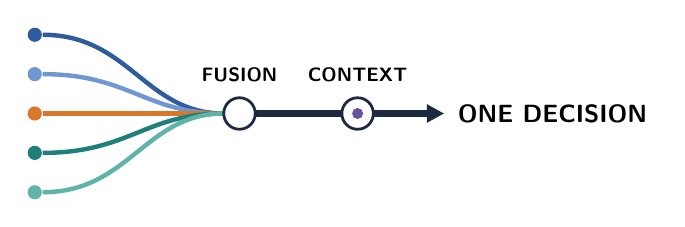
\begin{tikzpicture}[x=1cm, y=1cm]
  \foreach \c/\i in {blue/0, bluelight/1, orange/2, teal/3, seagreen/4}{\fill[\c] (0, 1.0-0.5*\i) circle (0.09); \draw[\c, line width=1.6pt] (0.1, 1.0-0.5*\i) .. controls (1.2, 1.0-0.5*\i) and (1.4, 0) .. (2.4, 0);}
  \draw[ink, fill=white, line width=1pt] (2.6, 0) circle (0.2); \node[anchor=south, font=\fontsize{7.5}{8}\selectfont\bfseries] at (2.6, 0.28) {FUSION};
  \draw[ink, line width=2.2pt] (2.8, 0) -- (3.9, 0); \draw[ink, fill=white, line width=1pt] (4.1, 0) circle (0.2); \fill[violet] (4.1, 0) circle (0.07); \node[anchor=south, font=\fontsize{7.5}{8}\selectfont\bfseries] at (4.1, 0.28) {CONTEXT};
  \draw[ink, line width=2.2pt, -{Triangle[length=2.2mm, width=2.2mm]}] (4.3, 0) -- (5.2, 0); \node[anchor=west, font=\latoblack\fontsize{9}{9}\selectfont] at (5.25, 0) {ONE DECISION};
\end{tikzpicture}}
% \sensorvisual[width]{file}: a generated figure
\newcommand{\sensorvisual}[2][\textwidth]{\includegraphics[width=#1]{#2}}
% \talk{script}{one sentence}{likely challenge}{answer}: speaker notes
\newcommand{\talk}[4]{\note{\textbf{Script.} #1\par\medskip\textbf{One sentence.} #2\par\medskip\textbf{Likely challenge.} #3\par\medskip\textbf{Answer.} #4}}
% \navytitle{...}: display type on the navy slides
\newcommand{\navytitle}[1]{{\latoblack\fontsize{26}{28}\selectfont\color{white}#1\par}}

% generated by make_slide_figures.py from docs/report/figures_src/*.json (and FACTS for Kaggle/organiser numbers); do not edit
\newcommand{\nFusedAcc}{0.781}
\newcommand{\nDecodedAcc}{0.830}
\newcommand{\nOracle}{2,399}
\newcommand{\nFusedClips}{2,109}
\newcommand{\nDecodedClips}{2,240}
\newcommand{\nOracleAcc}{0.889}
\newcommand{\nRescueSkel}{73}
\newcommand{\nRescueTherm}{68}
\newcommand{\nRescuePerson}{61}
\newcommand{\nRescueWrist}{52}
\newcommand{\nRescueImu}{34}
\newcommand{\nLooMin}{11}
\newcommand{\nLooMax}{48}
\newcommand{\nAllWrong}{301}
\newcommand{\nDistinct}{+55}
\newcommand{\nOrder}{+76}
\newcommand{\nDecoderGain}{+131}
\newcommand{\nShuffled}{+9}
\newcommand{\nReversed}{-54}
\newcommand{\nPermuted}{-17}
\newcommand{\nPersonA}{0.714}
\newcommand{\nPersonB}{0.733}
\newcommand{\nWristDelta}{-1.36}
\newcommand{\nThermA}{0.544}
\newcommand{\nThermB}{0.568}
\newcommand{\nThermC}{0.627}
\newcommand{\nThermGain}{+5.6}
\newcommand{\nThermPublic}{+5}
\newcommand{\nThermFusion}{46}
\newcommand{\nLosoPersonMean}{73.0}
\newcommand{\nLosoEnsMean}{78.2}
\newcommand{\nLosoPersonSd}{6.4}
\newcommand{\nLosoEnsSd}{5.4}
\newcommand{\nLosoPersonSpread}{23}
\newcommand{\nLosoEnsSpread}{21}
\newcommand{\nLosoUp}{14}
\newcommand{\nLosoN}{16}
\newcommand{\nWorstMissing}{-48}
\newcommand{\nWorstMissingPts}{-1.8}
\newcommand{\nCoefMin}{-24}
\newcommand{\nCoefMax}{+7}
\newcommand{\nVideoMB}{64.8}
\newcommand{\nSkelMB}{18.9}
\newcommand{\nDetMB}{10.3}
\newcommand{\nForestMB}{1.6}
\newcommand{\nTotalMB}{96.37}
\newcommand{\nFreeMB}{3.63}
\newcommand{\nGpus}{5}
\newcommand{\nMaxDrift}{2e-3}
\newcommand{\wPerson}{0.236}
\newcommand{\wWrist}{0.181}
\newcommand{\wThermal}{0.170}
\newcommand{\wSkel}{0.332}
\newcommand{\wImu}{0.297}
\newcommand{\wPrior}{0.25}
\newcommand{\fPrivate}{0.877}
\newcommand{\fPrivateClips}{179/204}
\newcommand{\fPublic}{0.866}
\newcommand{\fPublicClips}{174/201}
\newcommand{\fRank}{14}
\newcommand{\fTeams}{307}
\newcommand{\fClasses}{40}
\newcommand{\fTrainSubjects}{18}
\newcommand{\fTrainClips}{2,933}
\newcommand{\fTestClips}{405}
\newcommand{\fBudget}{100}
\newcommand{\fTimeCluster}{2 min 39 s}
\newcommand{\fTimeLaptop}{4 min 53 s}
\newcommand{\fPeakGpu}{5.4}

\ifdefined\shownotes\setbeameroption{show notes on second screen=right}\fi
\title{Five Sensors. One Decision.}
\author{Team AGX}
\begin{document}

% ============================================================ 1  HERO
\begin{frame}[plain]
\begin{tikzpicture}[remember picture, overlay]
  \node[anchor=north west, inner sep=0] at ([xshift=0.6cm, yshift=-0.35cm]current page.north west) {\latoblack\fontsize{22}{22}\selectfont\color{ink}FIVE SENSORS.};
  \node[anchor=north west, inner sep=0] at ([xshift=0.6cm, yshift=-1.25cm]current page.north west) {\latoblack\fontsize{22}{22}\selectfont\color{blue}ONE DECISION.};
  \node[anchor=north east, inner sep=0, align=right] at ([xshift=-0.6cm, yshift=-0.42cm]current page.north east) {\fontsize{9.5}{11.5}\selectfont\bfseries\color{ink}Can a machine recognise everyday activities\\without an ordinary camera?};
  \node[anchor=north east, inner sep=0] at ([xshift=-0.6cm, yshift=-1.4cm]current page.north east) {\begin{tabular}{@{}r@{}}\fontsize{7}{8.5}\selectfont\color{graytext}Multimodal activity recognition under a 100 MB constraint\\\fontsize{7}{8.5}\selectfont\color{graytext}CUHK-X Challenge 2026\quad$\cdot$\quad Small Model Track\quad$\cdot$\quad Team AGX\end{tabular}};
  \node[anchor=north, inner sep=0] at ([yshift=-2.25cm]current page.north) {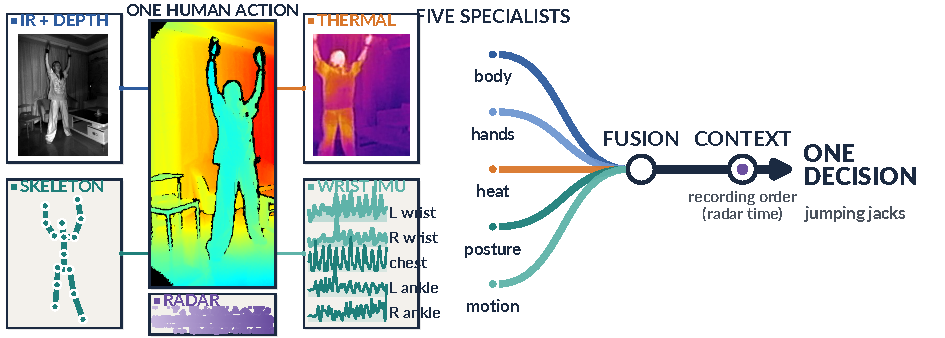
\includegraphics[width=14cm]{s01_hero.pdf}};
  \node[anchor=south, inner sep=0] at ([yshift=0.5cm]current page.south) {%
    \begin{tabular}{@{}c@{\hspace{1.1cm}}c@{\hspace{1.1cm}}c@{\hspace{1.1cm}}c@{}}
      {\latoblack\fontsize{15}{15}\selectfont\fClasses} & {\latoblack\fontsize{15}{15}\selectfont\nTotalMB\,MB} & {\latoblack\fontsize{15}{15}\selectfont\fPrivate} & {\latoblack\fontsize{15}{15}\selectfont UNSEEN}\\[1pt]
      {\fontsize{7}{8}\selectfont\color{graytext}\bfseries ACTIVITIES} & {\fontsize{7}{8}\selectfont\color{graytext}\bfseries ONE FILE} & {\fontsize{7}{8}\selectfont\color{graytext}\bfseries PRIVATE SCORE} & {\fontsize{7}{8}\selectfont\color{graytext}\bfseries PEOPLE AT TEST TIME}\\
    \end{tabular}};
  \node[anchor=south, inner sep=0] at ([yshift=0.16cm]current page.south) {\fontsize{6.5}{7}\selectfont\color{graytext}\fRank th of \fTeams\ teams\quad$\cdot$\quad 0 / \fTestClips\ predictions changed across \nGpus\ tested GPU generations\quad$\cdot$\quad no network at inference};
\end{tikzpicture}
\talk{This is one training clip, jumping jacks, seen by the depth camera. No face is recorded. The same instant reaches the system through five different lenses: infrared and depth, thermal, a tracked skeleton, wrist and body inertial units, and radar. Five small specialists each read one of those streams; their votes are fused, the order of the recording adds context, and out comes one decision: jumping jacks. Forty activities, one 96-megabyte file, people the model has never seen, 0.877 on the private leaderboard, and the same 405 predictions on every GPU we tested.}{One human action, seen five ways, fused into one decision by a system that fits in 96 MB.}{Why five sensors instead of one good camera?}{Because the task forbids an ordinary camera, and because, as slide 3 shows, the five streams make different mistakes: 2,399 of 2,700 held-out clips are right for at least one specialist, and no single one reaches 0.75.}
\end{frame}

% ============================================================ 2  THE PROBLEM
\begin{frame}{WHAT IF THE CAMERA NEVER SAW YOUR FACE?}
\takeaway{Recognise forty everyday activities from sensors that cannot identify anyone, for people the model has never seen, with the whole system in one file of at most 100 MB.}
\begin{columns}[T]
\column{0.42\textwidth}\centering\sensorvisual[6.2cm]{s02_layers.pdf}
\column{0.58\textwidth}
\vspace{0.1cm}
\begin{columns}[T]
\column{0.30\linewidth}\heronum[22]{\fClasses}{ACTIVITIES}
\column{0.30\linewidth}\heronum[22]{\fTrainSubjects}{TRAINING SUBJECTS}
\column{0.40\linewidth}\heronum[22]{\fBudget\,MB}{MAXIMUM, ONE FILE}
\end{columns}
\vspace{0.45cm}
{\latoblack\fontsize{11.5}{13.5}\selectfont Generalise to people the model has never seen.\par}
\vspace{0.35cm}
{\fontsize{8.5}{11}\selectfont\color{graytext}
\fTrainClips\ training clips from \fTrainSubjects\ people; \fTestClips\ test clips from 4 unseen people.\\[3pt]
Infrared + depth, thermal, 17-joint skeleton, five inertial units, radar. No RGB camera anywhere in the data.\\[3pt]
Scored on those new people, on reproducibility and on efficiency: cross-subject robustness is worth more than the leaderboard.\par}
\vspace{0.15cm}
{\fontsize{7.5}{9}\selectfont\color{graytext}\bfseries \fTestClips\ test clips\quad$\cdot$\quad unseen people\quad$\cdot$\quad additional held-out subjects\par}
\end{columns}
\talk{The setting is a home or a care room where an ordinary camera is unwelcome, because identity must not be recorded. So the sensors are ones that see a body, heat, joints and motion, not a face. The catch is threefold: forty fine-grained activities, only eighteen people to learn from, and a single file of at most 100 megabytes. And the score that matters most is measured on people the model has never seen.}{Privacy-preserving sensors, unseen people, a 100 MB budget: the constraints define the problem.}{Isn't an infrared camera just a camera?}{It is a body-shaped image, not a face-resolving one, and the depth channel we lead with carries no identity at all; the benchmark's definition of privacy-preserving is the organisers', and every stream we use is one they provide.}
\end{frame}

% ============================================================ 3  COMPLEMENTARITY (hero)
\begin{frame}{ONE SENSOR SEES ONLY PART OF THE STORY.}
\takeaway{Every one of 2,700 held-out training clips, coloured by which specialists classify it correctly.}
\centering\sensorvisual[14.8cm]{s03_field.pdf}
\vspace{0.05cm}
\begin{columns}[T]
\column{0.34\textwidth}\heronum[20]{\nOracle\ / 2,700}{correct for at least one specialist (\nOracleAcc)}
\column{0.30\textwidth}\vspace{0.05cm}{\latoblack\fontsize{10.5}{12.5}\selectfont Different sensors make different mistakes.\par}
\column{0.34\textwidth}\raggedleft{\fontsize{7.5}{9}\selectfont\color{graytext}\bfseries REMOVE ANY ONE MEMBER\par}{\latoblack\fontsize{15}{15}\selectfont\color{red}$-$\nLooMin\ TO $-$\nLooMax\ CLIPS\par}{\fontsize{7.5}{9}\selectfont\color{graytext}every specialist is load-bearing\par}
\end{columns}
\talk{Each square here is one held-out clip. Navy: all five specialists get it right. Grey: some do. The coloured stripe is the interesting part: 288 clips that exactly one specialist gets right, and every colour is there. The skeleton alone rescues 73, thermal 68, the body view 61, the hands 52, even the motion forest 34. Add them up and at least one specialist is right on 2,399 of 2,700 clips, 0.889, while the best single one is at 0.733. The information is in the members; the problem is selecting it. And removing any member costs the fusion between 11 and 48 clips.}{Different sensors make different mistakes, so the union is far larger than any one of them.}{Why keep the weakest member, the forest at 0.377?}{It is the only member right on 34 clips, removing it costs 11, and its paired per-subject effect is neutral at worst; it also costs 1.6 MB.}
\end{frame}

% ============================================================ 4  THE CORE IDEA
\begin{frame}{FIVE SPECIALISTS. ONE DECISION.}
\takeaway{Each specialist reads the stream it is built for; a prior-corrected log-linear sum fuses their votes; the recording's order adds context.}
\centering\sensorvisual[15.4cm]{s04_converge.pdf}
\talk{Here is the whole system in one motion. The body view and the hand view are two MViTv2-S video models on the infrared and depth crops; the heat view is the same architecture on the thermal full frame; posture is a twenty-member skeleton and inertial ensemble; motion is a small tree forest on wrist statistics. Their posteriors are combined as a weighted sum of log-probabilities, the coefficients chosen by nested cross-validation, which takes 2,700 held-out clips from 0.733 for the best member to 0.781. Then the ordered transition decoder uses the order of a recording session, which the radar timestamps give us, to reach 0.830.}{Complementary small specialists plus the structure of the recording, not model size.}{Why fuse in log space with a prior correction?}{The video members are trained with a prior-corrected loss and emit uniform-prior posteriors, the skeleton ensemble emits train-prior posteriors; we divide the latter by the prior before summing. Getting the direction wrong cost four points on an early submission: 0.587 versus 0.627.}
\end{frame}

% ============================================================ 5  RESOLUTION
\begin{frame}{MORE PIXELS ARE NOT ALWAYS MORE INFORMATION.}
\takeaway{Resolution helps the body crop up to 384 px and hurts the wrist crop already at 288 px; the difference is what one input pixel contains.}
\centering\sensorvisual[15.4cm]{s05_resolution.pdf}
\vspace{0.05cm}
{\latoblack\fontsize{10}{11}\selectfont Resolution pays where the crop contains real detail.\par}
\talk{The person crop climbs from 0.714 at 224 pixels to 0.733 at 384, four folds out of four, and falls back at 448. The wrist crop does the opposite: from 224 to 288 it loses 1.36 points, three folds out of four. The reason is on the right. A person box spans 224 to 480 source pixels, so a 384-pixel input samples detail the frame really has. A wrist box is about 96 source pixels, so at 288 each source pixel becomes nine input pixels of interpolation. More pixels, no more information.}{Resolution is crop-dependent: it pays where the crop contains real detail.}{Did you test beyond 384?}{Yes: 448 is measured, minus 0.81 on the member and minus 17 fused clips with t = minus 2.0; not shipped.}
\end{frame}

% ============================================================ 6  THERMAL
\begin{frame}{THERMAL WAS USELESS. UNTIL WE READ IT CORRECTLY.}
\takeaway{The same camera, three recipes: a 128 px person crop, the 128 px full frame, the 224 px full frame through the video recipe.}
\centering\sensorvisual[15.2cm]{s06_thermal.pdf}
\vspace{0.02cm}
{\latoblack\fontsize{12}{13}\selectfont SAME SENSOR. DIFFERENT WAY OF READING IT.\par}
\talk{Thermal is the dataset paper's strongest single sensor, yet our first thermal member, a 128-pixel person crop through a 3-D CNN, scored 0.544 and added exactly nothing in fusion at any weight. Reading the full frame at 128 pixels gave 0.568, still not adopted. Reading the full frame at 224 pixels through the same MViTv2-S recipe as the video members gave 0.627, plus 5.6 points on four folds out of four, and for the first time thermal helped the system: 46 more decoded clips out of 2,700 and 5 more public clips. The camera never changed. The 320 by 240 frame is read near-natively, and the objects and the room stay in view.}{Thermal became a contributing sensor when it was read at native resolution with the objects in view.}{Why was it useless before, if the sensor is strong?}{Wrong recipe for the sensor: cropping removed the objects that define most classes, and 128 pixels threw away most of the frame. Decorrelation alone did not make it useful; accuracy did.}
\end{frame}

% ============================================================ 7  GENERALISATION
\begin{frame}{THE REAL TEST IS THE PERSON YOU'VE NEVER SEEN.}
\takeaway{Leave one training subject out, fit the rest, score the held-out person: the person view alone against the shipped ensemble, paired on \nLosoN\ subjects.}
\begin{columns}[T]
\column{0.70\textwidth}\sensorvisual[11.3cm]{s07_subjects.pdf}
\column{0.29\textwidth}
\vspace{0.1cm}
\heronum[18]{\nLosoPersonMean\ $\rightarrow$ \nLosoEnsMean}{mean accuracy over \nLosoN\ held-out subjects}
\vspace{0.2cm}
\heronum[12.5]{sd \nLosoPersonSd\ $\rightarrow$ \nLosoEnsSd}{the subjects become more alike}
\vspace{0.2cm}
\heronum[12.5]{spread \nLosoPersonSpread\ $\rightarrow$ \nLosoEnsSpread}{points, hardest to easiest person}
\vspace{0.2cm}
\resultbadge{\nLosoUp\ / \nLosoN\ subjects improve}\par
\vspace{0.25cm}
{\fontsize{7.5}{9}\selectfont\color{graytext}An 18-subject leave-one-subject-out run supports the direction; the organisers' additional held-out subjects remain the final external test.\par}
\end{columns}
\talk{Subjects, not clips, are the unit of generalisation here, so we hold out one person at a time. Grey is the person view alone; navy is the shipped ensemble; each vertical line is one held-out person. Fourteen of sixteen go up, the mean goes from 73.0 to 78.2, and the spread between the hardest and the easiest person narrows from 23 points to 21. The two that go down are within seed noise. Fusion does not only raise accuracy; it makes the system more even across people, which is what the held-out evaluation rewards.}{Fusion raises fourteen of sixteen held-out people and makes them more alike.}{Leave-one-subject-out is not a new site.}{Agreed: it is sixteen draws of an unseen person, the closest measurement we have; a draw of eight subjects still carries about two points of standard error, which is why we do not oversell the leaderboard either.}
\end{frame}

% ============================================================ 8  ROBUSTNESS
\begin{frame}{WHAT HAPPENS WHEN A SENSOR DISAPPEARS?}
\takeaway{The frozen fusion under two kinds of damage: a sensor absent, or one coefficient scaled by half to one and a half; every cell is the change in fused OOF clips.}
\begin{columns}[T]
\column{0.66\textwidth}\sensorvisual[9.7cm]{s08_atlas.pdf}
\column{0.33\textwidth}
\vspace{0.1cm}
\heronum[26]{\nWorstMissing}{CLIPS: worst single-sensor loss (\nWorstMissingPts\ points, the body view)}
\vspace{0.35cm}
\heronum[18]{\nCoefMin\ TO \nCoefMax}{all coefficient perturbations, $\times$0.5 to $\times$1.5}
\vspace{0.3cm}
{\fontsize{7.5}{9}\selectfont\color{graytext}any re-weighting moves at most 8 of the 405 test rows\par}
\end{columns}
\vspace{-0.1cm}
{\latoblack\fontsize{10.5}{12}\selectfont THE FUSION SITS ON A PLATEAU, NOT A PEAK.\par}
\talk{This is a reliability test, not an ablation for its own sake. Remove any sensor at inference, the way the pipeline really handles a missing stream, and the worst case is the body view: 48 clips of 2,700, 1.8 points. Thermal and the forest cost eleven to twelve. Scale any fusion coefficient by half or by one and a half, and the fused accuracy stays within minus 24 to plus 7 clips, under one percent. No sensor is a single point of failure and the coefficients are on a plateau.}{No single point of failure; the coefficients sit on a plateau.}{Did you fit the weights to the leaderboard?}{No: nested cross-validation inside the folds; and the plateau shows it would not matter, at most 8 of 405 rows move under any re-weighting.}
\end{frame}

% ============================================================ 9  STRUCTURE
\begin{frame}{THE RECORDING ITSELF KNOWS SOMETHING.}
\takeaway{A recording session is a script of distinct activities in a fixed order; the decoder uses that order, learned from training metadata only, never from test labels.}
\centering\sensorvisual[15.4cm]{s09_waterfall.pdf}
\vspace{0.05cm}
{\fontsize{8.5}{10}\selectfont\color{graytext}Label-free, and neutral without structure: shuffled \nShuffled, reversed \nReversed, permuted labels \nPermuted.\par}
\talk{The fused argmax gets 2,109 clips right. The first thing the recording tells us is that its activities are distinct: a soft penalty on repeating a label within a session adds 55. The second is the scripted order: a first-order transition model over classes, fitted on training metadata, adds 76 more through beam search. That is 2,240, plus 131 clips, and the same decoder gave plus three to five clips on the public leaderboard. The controls on the right are what make this science rather than a trick: shuffle the order within sessions and the gain is plus 9, neutral; reverse it and it is minus 54; permute the class labels and it is minus 17. The decoder is reading structure, not memorising label frequencies.}{Recording structure carries measurable information, and the controls show it is structure, not memorisation.}{You are exploiting the recording order.}{It is label-free, fitted on training metadata only, and neutral when the order is absent: a clip without a radar key simply gets the fused argmax.}
\end{frame}

% ============================================================ 10  WHAT FAILED
\begin{frame}{SO WE TRIED THE OBVIOUS THINGS.}
\takeaway{Every lever measured against the same bar: paired folds, two standard errors (seed sd 1.16 points). Red was rejected, blue adopted.}
\centering\sensorvisual[14.2cm]{s10_levers.pdf}
\vspace{0.05cm}
{\latoblack\fontsize{10}{11}\selectfont The bottleneck was not simply model capacity.\par}
\talk{We tried the obvious things first. More capacity: VideoMAE-B with 87 million parameters lost 1.8 points on zero of four folds, Swin3D-T lost 9.8, a V-JEPA 2 teacher was 29 points behind. More training tricks: layer-wise decay was noise, distillation and self-training helped a member and hurt the fusion. More test-time tricks: temporal augmentation, seed soups, a pair verifier, all negative or unreadable. Resolution was mixed, and that is the honest version: 288 and 384 on the body helped, 448 and the wrist step did not. What worked was a different kind of information: a new sensor view, fusing in the right space, and the structure of the recording.}{More of the same did not help; a different kind of information did.}{Isn't MViTv2-S itself a capacity upgrade?}{It replaced a similar-sized 3-D CNN, plus 2.4 points at 34 million parameters; the larger models above it all lost. Capacity beyond that point overfits 2,281 training clips.}
\end{frame}

% ============================================================ 11  100 MB
\begin{frame}{WE FIT AN ENTIRE SYSTEM INTO 100 MB.}
\takeaway{The budget was an architectural constraint, not a compression exercise: which members to keep, at which precision, with both detectors inside.}
\centering\sensorvisual[14.6cm]{s11_container.pdf}
\begin{columns}[T]
\column{0.34\textwidth}\heronum[22]{\nTotalMB\ MB}{every inference-time weight inside}
\column{0.64\textwidth}\vspace{0.05cm}\callout{Video 5-bit, ensemble int8, detectors fp16. \textbf{int8 detectors moved 150 of 405 crop windows}, so they stay fp16; int5 video cost one public clip against int6.}
\end{columns}
\talk{The container is the 100-megabyte rule. Three video models at five-bit weight codes take 64.8 megabytes, two thirds of it. The skeleton and inertial ensemble, pruned from 48 members to 20 and stored at int8, takes 18.9. Both detectors, 10.3 megabytes at fp16, plus the forest, the crop windows and the manifest. 96.37 megabytes, 3.6 to spare. Two decisions were measured, not assumed: five-bit video cost one public clip against six-bit, recovered elsewhere; and quantising the detectors to int8 would have moved 150 of 405 crop windows, so they stayed at fp16.}{Everything the system needs at inference lives in one 96.37 MB file, and every byte was a measured trade-off.}{Where are the detectors?}{Inside the file, fp16, 10.3 MB; the 405 crop windows are stored too, so the Kaggle run is reproduced exactly, and new data goes through the live detectors.}
\end{frame}

% ============================================================ 12  REPRODUCIBILITY
\begin{frame}{AND IT ACTUALLY RUNS.}
\takeaway{One command, no network, data read-only, verified from the uploaded archives in a clean room, on \nGpus\ GPU generations.}
\begin{columns}[T]
\column{0.22\textwidth}
{\fontsize{7.5}{9}\selectfont\color{graytext}\bfseries ONE COMMAND\par}\vspace{3pt}
\colorbox{ink}{\parbox{\dimexpr\linewidth-2\fboxsep\relax}{\color{white}\ttfamily\bfseries\fontsize{8}{10}\selectfont bash inference.sh <data> <out.csv>}}
\vspace{0.3cm}
\heronum[13]{\fTimeCluster}{for all \fTestClips\ clips on an A100; \fTimeLaptop\ on a laptop RTX 4060; peak GPU memory \fPeakGpu\ GB}
\column{0.50\textwidth}
\centering{\fontsize{7.5}{9.5}\selectfont% generated by make_slide_figures.py from gpu.json; do not edit
\begin{tabular}{@{}l l c c@{}}\toprule
\textbf{GPU} & \textbf{posterior drift} & \textbf{predictions} & \textbf{CSV}\\
 & {\color{graytext}video / skeleton} & {\color{graytext}changed} & \\\midrule
\vrowc{RTX 4060}{reference}{0 / 405}{IDENTICAL}
\vrowc{A100}{1.6e-3 / 4.4e-5}{0 / 405}{IDENTICAL}
\vrowc{H100}{2.0e-3 / 4.3e-5}{0 / 405}{IDENTICAL}
\vrowc{H200}{2.0e-3 / 4.3e-5}{0 / 405}{IDENTICAL}
\vrowc{V100}{1.7e-3 / 9.2e-5}{0 / 405}{IDENTICAL}
\bottomrule\end{tabular}
\par}
\column{0.26\textwidth}
{\latoblack\fontsize{10}{11.5}\selectfont NUMERICAL DRIFT EXISTS.\par THE DECISION DOES NOT MOVE.\par}
\vspace{0.3cm}
\heronum[20]{0 / \fTestClips}{predictions changed on \nGpus\ GPU generations; posteriors drift up to \nMaxDrift}
\end{columns}
\vspace{0.35cm}
\centering\okbadge{NETWORK OFF}\quad\okbadge{READ-ONLY DATA}\quad\okbadge{HOSTILE TESTS}\quad\okbadge{CLEAN ROOM $\times$2}\par
\vspace{0.15cm}
{\fontsize{7}{8.5}\selectfont\color{graytext}second selected submission byte-identical; primary reproduced 403/405 after the skeleton ensemble was pruned to fit 100 MB, the two decoder near-ties disclosed, not fitted (backup B8)\par}
\talk{The package is one command: no arguments beyond the data directory and the output path, no network, the data mounted read-only. We verified it from the actual uploaded archives in a clean room, twice, with the working repository moved aside. Then we ran the same container on five GPU generations. Posteriors drift by up to two in a thousand, the way half-precision arithmetic does; the argmax changes on zero of 405 clips and the CSV is byte-identical every time. That is the claim: not bitwise determinism, but a decision that does not move.}{Numerical drift exists; the decision does not move, on five GPU generations, from the uploaded archives.}{Your primary submission reproduces 403 of 405, not 405.}{Yes, and we say so. The skeleton ensemble was pruned from 48 to 20 members after that submission to meet the size rule; two decoder near-ties flip. About 900 coefficient settings were tried and none closer, so we ship the principled coefficients and disclose the two rows rather than fit to the target file. The second submission is byte-identical.}
\end{frame}

% ============================================================ 13  TAKEAWAY (navy)
{\setbeamercolor{background canvas}{bg=ink}\setbeamercolor{normal text}{fg=white}
\begin{frame}[plain]
\begin{tikzpicture}[remember picture, overlay]
  \node[anchor=north west, inner sep=0] at ([xshift=0.8cm, yshift=-0.9cm]current page.north west) {\latoblack\fontsize{27}{27}\selectfont\color{white}FIVE SENSORS.};
  \node[anchor=north west, inner sep=0] at ([xshift=0.8cm, yshift=-1.95cm]current page.north west) {\latoblack\fontsize{27}{27}\selectfont\color{bluelight}ONE DECISION.};
  \node[anchor=north west, inner sep=0] at ([xshift=0.8cm, yshift=-3.55cm]current page.north west) {%
    \begin{tabular}{@{}l@{\hspace{1.0cm}}l@{\hspace{1.0cm}}l@{\hspace{1.0cm}}l@{}}
      {\latoblack\fontsize{21}{21}\selectfont\color{white}\fClasses} & {\latoblack\fontsize{21}{21}\selectfont\color{white}\nTotalMB\,MB} & {\latoblack\fontsize{21}{21}\selectfont\color{white}\fPrivate} & {\latoblack\fontsize{21}{21}\selectfont\color{white}UNSEEN}\\[2pt]
      {\fontsize{8}{9}\selectfont\color{graylight}\bfseries ACTIVITIES} & {\fontsize{8}{9}\selectfont\color{graylight}\bfseries ONE FILE} & {\fontsize{8}{9}\selectfont\color{graylight}\bfseries PRIVATE, \fRank th OF \fTeams} & {\fontsize{8}{9}\selectfont\color{graylight}\bfseries PEOPLE}\\
    \end{tabular}};
  \node[anchor=north west, inner sep=0] at ([xshift=0.8cm, yshift=-5.35cm]current page.north west) {\begin{tabular}{@{}l@{}}\latoblack\fontsize{15}{17}\selectfont\color{white}THE NEXT GAIN IS MORE SUBJECTS,\\\latoblack\fontsize{15}{17}\selectfont\color{white}NOT MORE MODEL.\end{tabular}};
  \node[anchor=south east, inner sep=0] at ([xshift=-0.8cm, yshift=0.75cm]current page.south east) {\latoblack\fontsize{14}{14}\selectfont\color{white}Team AGX};
  \node[anchor=south east, inner sep=0] at ([xshift=-0.8cm, yshift=0.35cm]current page.south east) {\fontsize{7.5}{8}\selectfont\color{graylight}CUHK-X Challenge 2026\quad$\cdot$\quad Small Model Track\quad$\cdot$\quad Atharv, BITS Pilani, K K Birla Goa Campus};
  \node[anchor=south west, inner sep=0] at ([xshift=0.8cm, yshift=0.4cm]current page.south west) {\begin{tikzpicture}[x=0.55cm, y=0.55cm]\foreach \c/\i in {blue/0, bluelight/1, orange/2, teal/3, seagreen/4}{\fill[\c] (0, 2.0-0.5*\i) circle (0.11); \draw[\c, line width=1.8pt] (0.12, 2.0-0.5*\i) .. controls (1.3, 2.0-0.5*\i) and (1.6, 1.0) .. (2.6, 1.0);}\draw[white, line width=2.6pt] (2.6, 1.0) -- (4.2, 1.0);\draw[white, line width=2.6pt, -{Triangle[length=2.4mm, width=2.4mm]}] (4.2, 1.0) -- (5.0, 1.0);\end{tikzpicture}};
\end{tikzpicture}
\talk{Five sensors, one decision. Ninety-six megabytes, forty activities, people the model has never seen, 0.877 private. The residual error we are left with is per-subject and correlated: twin recordings of the same person share the identical wrong label 68 percent of the time, and no lever that assumes independent evidence reaches it. So the next gain is more subjects, not more model. We froze the competitive solution, reproduced it, stress-tested it, and measured what actually mattered. Thank you.}{Complementary small specialists plus structure beat model size, and the limits are measured too.}{What would you do with a month?}{Subject diversity in representation learning, tested the same way: paired folds, a two-standard-error bar, and a per-subject delta, because a frozen-feature probe saturates at six subjects and any gain must come through the representation.}
\end{frame}}

% ============================================================ BACKUP
\begin{frame}[plain]
\vspace{2.8cm}\centering{\latoblack\fontsize{22}{22}\selectfont\color{ink}BACKUP\par}\vspace{0.2cm}{\fontsize{9}{11}\selectfont\color{graytext}architecture $\cdot$ fusion $\cdot$ members $\cdot$ the full landscape $\cdot$ subjects $\cdot$ decoder $\cdot$ package $\cdot$ limitations and disclosure\par}
\end{frame}

\begin{frame}{B1 \ THE SYSTEM, IN FULL}
\takeaway{Five streams, five specialists, one file (report Fig. 1). Member accuracies are pooled OOF over 2,700 clips of held-out subjects; the card's \fPrivate\ is the Kaggle private score.}
\centering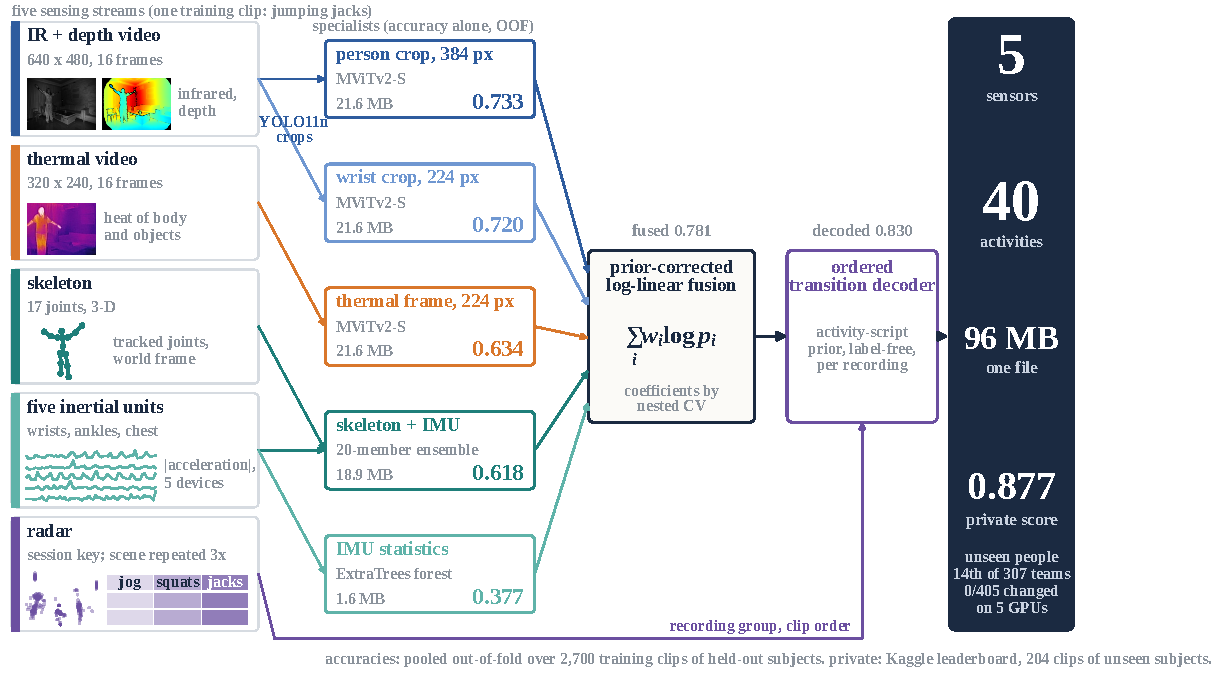
\includegraphics[width=10.4cm]{fig01_abstract.pdf}
\talk{The report's first figure: every sensing stream on the left as this clip sees it, the five specialists with their size and accuracy, the fusion, the decoder, and the result card.}{The whole system on one page.}{How large is each member?}{Three MViTv2-S at 21.6 MB each in 5-bit codes, the 20-member skeleton/IMU ensemble at 18.9 MB in int8, the forest at 1.6 MB; the detectors 10.3 MB in fp16.}
\end{frame}

\begin{frame}{B2 \ FUSION: THE RIGHT PROBABILITY SPACE}
\begin{columns}[T]
\column{0.5\textwidth}
\callout{\textbf{Members are combined as} $\sum_i w_i \log p_i$. Video members are trained with a prior-corrected loss and emit \textbf{uniform-prior} posteriors; the skeleton ensemble is trained with plain cross-entropy and emits \textbf{train-prior} posteriors, so it is divided by the training prior before the sum. The direction is measured: the wrong way cost 4 points on an early submission pair (0.587 vs 0.627).}
\vspace{0.3cm}
{\fontsize{8.5}{11}\selectfont
\begin{tabular}{@{}l r@{}}
\toprule \textbf{coefficient} & \textbf{shipped}\\ \midrule
person (body) & \wPerson\\ wrist (hands) & \wWrist\\ thermal (heat) & \wThermal\\ skeleton/IMU (posture) & \wSkel\\ IMU forest (motion) & \wImu\\ class prior & \wPrior\\ \bottomrule
\end{tabular}\par}
\column{0.48\textwidth}
{\fontsize{8.5}{11}\selectfont Coefficients are the centroid of the top-25 settings of a nested cross-validation over a 768-point grid, which reproduces the nested-CV estimate without the selection optimism of the argmax. The stability atlas (slide 8, report Fig. 7) shows the plateau: every coefficient $\times$0.5 to $\times$1.5 stays within \nCoefMin\ to \nCoefMax\ clips.\par}
\vspace{0.3cm}
\centering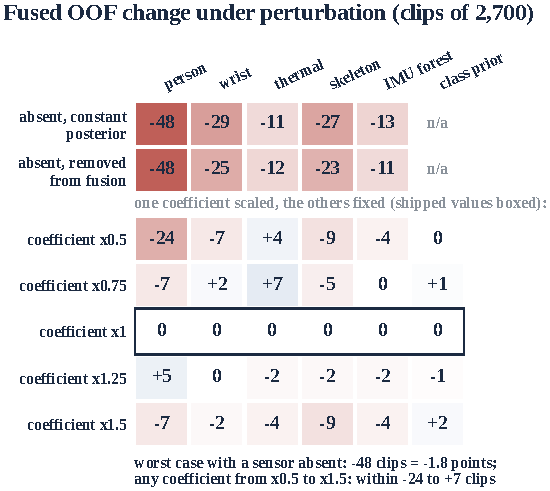
\includegraphics[width=4.4cm]{fig06_robustness.pdf}
\end{columns}
\talk{The fusion is a weighted sum of log posteriors with one twist: the members live in different prior spaces, and the skeleton ensemble must be divided by the training prior first. The coefficients come from nested cross-validation and sit on a plateau.}{Fuse in the right prior space; the coefficients are a plateau, not a fit.}{Why not learn a fusion network?}{Every learned selector we tried, a verifier, alignment, an object probe, failed to recover the oracle's 2,399 from the posteriors; with 2,700 clips a six-coefficient plateau is the honest amount of fitting.}
\end{frame}

\begin{frame}{B3 \ WHY FIVE MEMBERS}
\takeaway{Report Fig. 2: all 2,700 OOF clips grouped by which members classify them correctly; leave-one-member-out on the same posteriors.}
\centering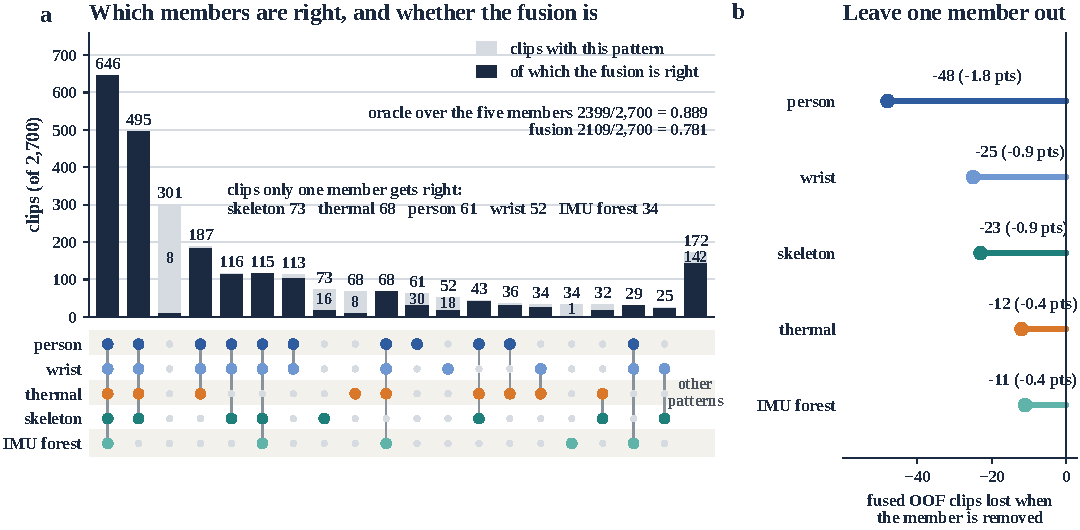
\includegraphics[width=13.2cm]{fig02_complementarity.pdf}
\talk{The full pattern table behind slide 3: 646 clips right for everyone, 301 wrong for everyone, 288 right for exactly one member; and the leave-one-out bars, person minus 48 down to the forest minus 11.}{Every member is load-bearing and the union is far larger than any member.}{Why not more members?}{Adding members to the video slot is a measured graveyard: four person folds and one person plus one wrist both reach the same public score; the budget is better spent on a new view than on a fifth copy of an old one.}
\end{frame}

\begin{frame}{B3b \ THE SKELETON / IMU ENSEMBLE}
\takeaway{What the posture specialist reads: the tracked skeleton and the five inertial units of the same clip.}
\centering\sensorvisual[12.2cm]{s12_ensemble.pdf}
\vspace{0.05cm}
\begin{columns}[T]
\column{0.2\textwidth}\heronumc[20]{20}{MEMBERS}
\column{0.2\textwidth}\heronumc[20]{5}{FAMILIES $\times$ 4 FOLDS}
\column{0.2\textwidth}\heronumc[20]{\nSkelMB\ MB}{INT8, ONE TENSOR SET}
\column{0.36\textwidth}{\fontsize{7.5}{9}\selectfont\color{graytext}adaptive-graph ST-GCN and ST-GCN on joints; a temporal CNN on joint, velocity and bone features; two temporal CNNs on the inertial units (rotation-invariant features; gravity-aligned world frame, no absolute orientation)\par}
\end{columns}
\talk{The posture specialist is not one model but twenty: five families, each trained on four subject-grouped folds, on the skeleton track and the inertial units you see here. Stored at int8 it is 18.9 megabytes, a fifth of the budget.}{Twenty small models on the skeleton and inertial streams, 18.9 MB.}{Why an ensemble here and single models for video?}{The skeleton members are small, so twenty of them cost 19 MB, and their fold diversity is what makes the ensemble's posterior calibrated enough to fuse; a video member is 21.6 MB each, so there the budget buys views, not seeds.}
\end{frame}

\begin{frame}{B4 \ THE FULL EXPERIMENT LANDSCAPE}
\takeaway{Report Fig. 9: every lever on one axis at the level it was measured (circle = member points, diamond = system clips / 27), with the adoption band.}
\centering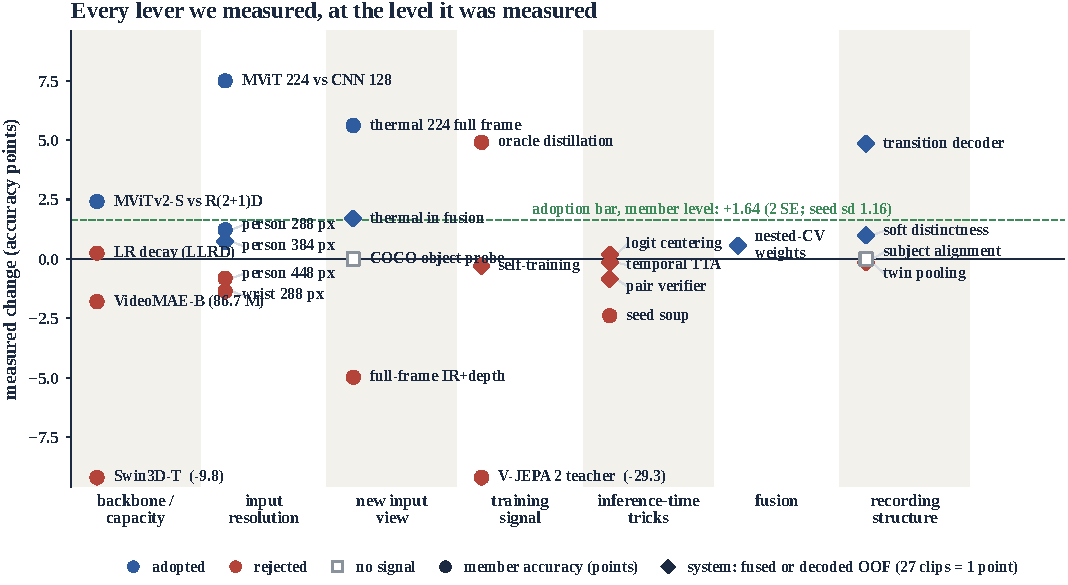
\includegraphics[width=11.2cm]{fig08_landscape.pdf}
\talk{Everything from slide 10 plus the levers that did not fit there: the backbone change, the full-frame IR duplicate, the COCO object probe, twin pooling, subject alignment.}{Twenty-five levers, one bar, one map.}{Why so many failures?}{They are the map; each was measured against a two-standard-error bar and recorded with its experiment id in the log.}
\end{frame}

\begin{frame}{B5 \ SUBJECT-LEVEL DETAIL}
\takeaway{Report Fig. 6: the paired 16-subject comparison and the distributions (mean, $\pm$1 sd, range).}
\centering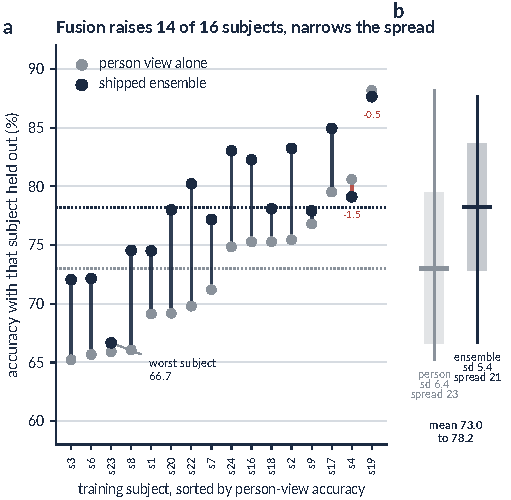
\includegraphics[width=14.0cm]{fig05_subjects.pdf}
\vspace{0.1cm}
{\fontsize{8}{10}\selectfont\color{graytext}Over all 18 subjects the person view has sd 6.9 and spread 28 (two subjects lack an ensemble value). Standard error of an 8-subject draw, which is what the private and held-out stages are: 2.4 $\rightarrow$ 1.9 points.\par}
\talk{The same slope pairs with the distribution strip, and the standard error of an eight-subject draw, which falls from 2.4 to 1.9 points.}{The dispersion falls as well as the mean.}{Are the two negative subjects a problem?}{Minus 1.5 and minus 0.5 points are inside seed noise of 1.16 per model; the paired mean delta is plus 5.2.}
\end{frame}

\begin{frame}{B6 \ DECODER CONTROLS}
\takeaway{Report Fig. 8: where the decoder's \nDecoderGain\ clips come from, and what happens when the structure is removed (rescued and harmed counted separately).}
\centering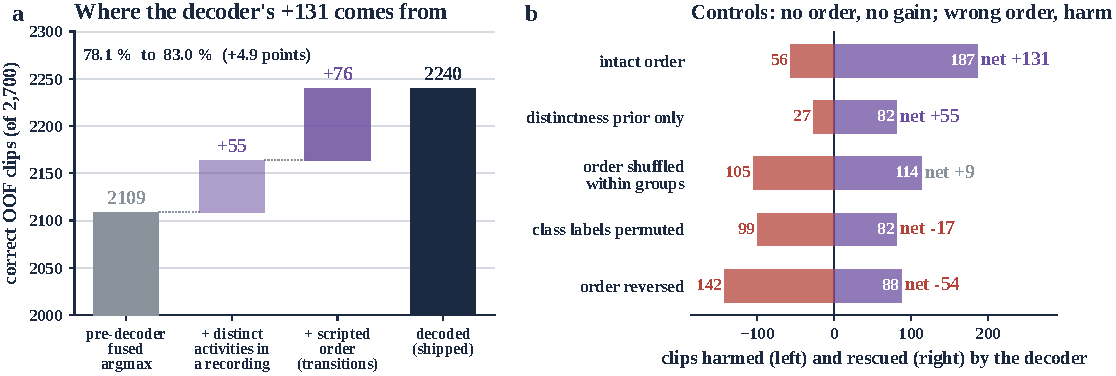
\includegraphics[width=13.0cm]{fig07_decoder.pdf}
\vspace{0.1cm}
{\fontsize{8}{10}\selectfont\color{graytext}Settings: transition weight 0.5, conditional transition scores with unigram back-off, soft distinctness penalty 2.0, beam search per recording group; a clip without a radar key receives the fused argmax.\par}
\talk{The decoder's gain decomposed and its controls with rescued and harmed counts: intact 187 rescued, 56 harmed; shuffled 114 and 105; reversed 88 and 142; permuted 82 and 99.}{The gain is structure, and the controls prove it.}{Would it work without radar?}{Without a session key the decoder is off by construction and the system returns the fused argmax, 0.781 OOF instead of 0.830.}
\end{frame}

\begin{frame}{B7 \ THE PACKAGE}
\begin{columns}[T]
\column{0.5\textwidth}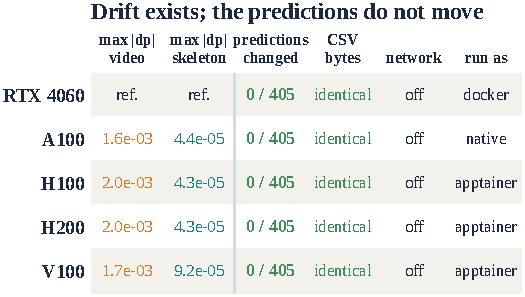
\includegraphics[width=\linewidth]{fig10_verification.pdf}
\column{0.48\textwidth}
{\fontsize{8.5}{11}\selectfont
\textbf{Archive} \texttt{small\_AGX\_verification\_v1.zip} (96.7 MB): \texttt{inference.sh}, \texttt{src/}, \texttt{artifacts/stage2\_ship7.pth} (\nTotalMB\ MB, sha256 recorded), \texttt{configs/} for both selected submissions, both CSVs byte-copied, README with the residual disclosure.\\[4pt]
\textbf{Image} \texttt{ghcr.io/atharvgaur1845/cuhkx-small-agx:v1} (public) and \texttt{image.tar.gz} (3.59 GB), \texttt{pytorch/pytorch:2.7.1-cuda12.6}.\\[4pt]
\textbf{Gates} G1 to G14: reproduction, offline, cache and id independence, synthetic hostile inputs (new ids, shuffled order, missing modalities, malformed files), docker with \texttt{--network none}, cross-GPU, content and secrets audit, clean-room from the uploaded archives with an independent comparer.\\[4pt]
\textbf{Timing} \fTimeCluster\ (A100), \fTimeLaptop\ (RTX 4060), peak GPU memory \fPeakGpu\ GB.\par}
\end{columns}
\talk{What the organisers received and how it was checked: the archive, the image, fourteen gates ending in a clean-room run from the uploaded files with a comparer that shares no code with the package.}{Verified from the actual upload, not from the working tree.}{What if the held-out data reuses the Kaggle clip ids?}{Crop windows are gated by a content fingerprint: a clip whose frames match the Kaggle clip uses the stored window, anything else goes through the live detectors; caches are per-run and wiped.}
\end{frame}

\begin{frame}{B8 \ LIMITATIONS AND DISCLOSURE}
\begin{columns}[T]
\column{0.56\textwidth}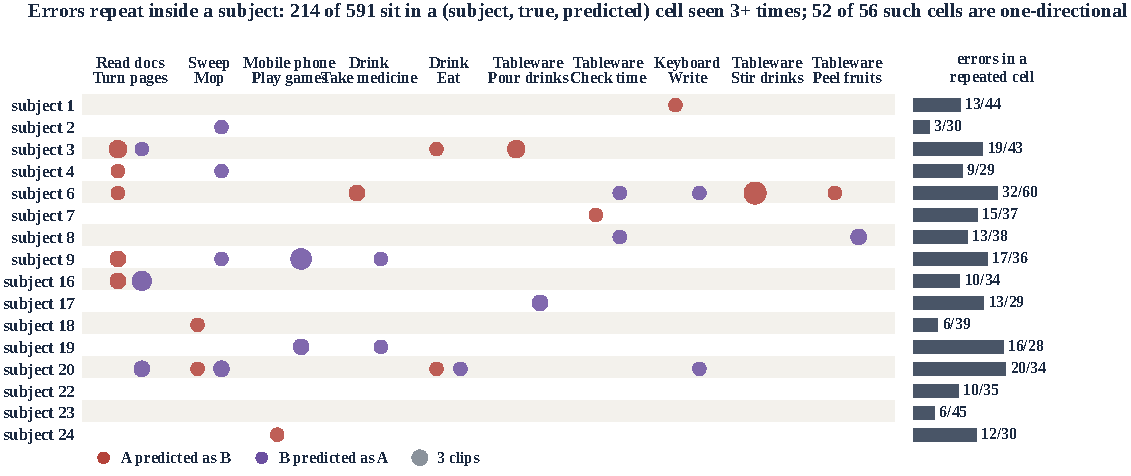
\includegraphics[width=\linewidth]{fig11_errors.pdf}
\vspace{0.2cm}
{\fontsize{7.5}{9}\selectfont\color{graytext}Report Fig. 10: 214 of 591 fused errors sit in a (subject, true, predicted) cell seen three or more times; 52 of 56 such cells are one-directional.\par}
\column{0.42\textwidth}
{\fontsize{8}{10}\selectfont
\textbf{The residual is subject-correlated.} Twin recordings share the identical wrong label 68\,\% of the time; no lever that assumes independent evidence reaches it.\\[4pt]
\textbf{More model: measured, no gain. More subjects:} the direction the evidence points to, not a quantified prediction (a frozen-feature probe saturates at six subjects).\\[4pt]
\textbf{Primary submission: 403/405.} The skeleton ensemble was pruned 48 $\rightarrow$ 20 after that submission to meet 100 MB; two decoder near-ties flip (margins 0.012 and 0.006). About 900 coefficient settings tried, none closer. We ship the principled coefficients and disclose the rows; the second submission is byte-identical.\\[4pt]
\textbf{Decoder dependence:} needs the recording key; neutral without it.\par}
\end{columns}
\talk{Where the errors are and why they are hard: they cluster by subject and by confusable object classes, read versus turn pages, sweep versus mop. The disclosure on the primary submission is here in full.}{The limits are measured and disclosed, not hidden.}{Why not fit the two rows?}{Because that would be fitting to the target file; the honour declaration and the verification guide both rule it out, and the two rows are worth less than the credibility of the package.}
\end{frame}

\end{document}
